\chapter{From Queries to a Submission, and How Good It Is}\label{ch:submission}

\section{Introduction}\label{sec:sub-intro}
\epigraph{Our judging committee will look at individual predictions, as well as the logic of the
algorithm.}{The competition's host, in the competition forum, 2026}

A trained network is not yet a submission. In this chapter we describe the path from the weights of
epoch 40 to the CSV file that the leaderboard scored (Section~\ref{sec:sub-path}), and the checks that
the deployment code performs before it writes any prediction (Section~\ref{sec:sub-replay}). We then
evaluate the resulting model: with the organisers' own scoring code (Section~\ref{sec:sub-eval}), by
looking at its predictions (Section~\ref{sec:sub-quality}), and by comparing it with the variants that
did not beat it (Section~\ref{sec:sub-variants}). We end with the next steps that our measurements
suggest (Section~\ref{sec:sub-next}).

\section{From weights to a CSV file}\label{sec:sub-path}
Between the weights of epoch 40 and the submitted file lie five steps, summarised in
Algorithm~\ref{alg:sub-emit}. Every one of them is shared, line for line, between validation and
deployment.

\begin{algorithmblock}{From a trained Mask2Former to a submission file\label{alg:sub-emit}}
\item \textbf{predict:} run the network on the native photograph in float32, and turn every query whose class probability exceeds a low floor (0.02) into a candidate, with a score from Equation~\eqref{eq:tr-score} and a binary mask of $2048\times2048$ pixels (Listing~\ref{lst:tr-predict});
\item \textbf{select:} keep the candidates whose score is at least the confidence threshold;
\item \textbf{paint:} give every pixel to the highest-scoring candidate that claims it, so that the masks become disjoint (Section~\ref{sec:masks-paint});
\item \textbf{filter:} drop the painted pieces that are smaller than the minimum area;
\item \textbf{encode:} write each remaining mask as a run-length encoding in one row of the CSV file (Section~\ref{sec:masks-rle})
\end{algorithmblock}

Listing~\ref{lst:sub-emit} shows the selection, painting and filtering steps as the code implements
them.

\begin{lstlisting}[caption={The emission rule, shared by validation and deployment. Condensed from
\file{experiments/exp\_139\_mask2former/src/submit.py:emit}.},label=lst:sub-emit]
def emit(entries, conf=0.85, grow=0, min_area=100):
    """exp033 sweep's emission, operation for operation, so the validated rule deploys unchanged."""
    candidates = []
    for entry in entries:                                   # entry: {score, rle}
        if entry["score"] < conf:
            continue
        mask = mu.decode(entry["rle"])
        if grow < 0:
            mask = cv2.erode(mask, KERNEL, iterations=-grow)   # never used by the final rule
        candidates.append((entry["score"], mask))
    painted = paint_panoptic(candidates, min_area=min_area)     # disjoint, highest score first
    return [encode(mask) for _, mask, _ in painted]
\end{lstlisting}

\subsection{Choosing the operating point}\label{sec:sub-operating}
The rule has three settings: the confidence threshold, an optional erosion, and the minimum area. We
chose them with the same sweep that we used to score every model in this book: 19 thresholds from 0.05
to 0.95, with and without a one-pixel erosion, and a minimum area of 100 or 300 pixels, making 76 rules
in all, each scored with the exact pooled PQ on the 180 validation records.

The sweep relies on a useful property of painting. Painting proceeds in order of decreasing score,
so raising the threshold only removes candidates from the \emph{end} of the painting order, and the
masks painted before them do not change. The set emitted at any threshold is therefore a prefix of the
set emitted at the lowest threshold, and all 19 thresholds can be scored from a single painting
(Exercise~\ref{ex:sub-prefix} asks for a proof). A unit test checks this equivalence.

The best rule for the final model used a threshold of 0.85, no erosion and a minimum area of 100
pixels. Two features of this rule fit what we know about the model. The threshold is high, which is
consistent with the calibration measurement of Section~\ref{sec:tta-calibration}, where we found the
Mask2Former's scores to be over-confident in the middle of their range. And the best erosion is none,
which is consistent with how its masks were trained: on \texttt{pycocotools} targets, which, unlike
the targets of the early YOLO models, are not systematically too wide.

\section{Replay before release}\label{sec:sub-replay}
The submission kernel ran on a free Kaggle T4. Before writing a single test prediction, it verified the
SHA-256 hash of the checkpoint against the manifest of the training run, re-checked the deformable
attention kernel on the T4, re-ran the validation with the deployment code, and required the result to
match the training run's validation score to within 0.005. The replay in float32 scored 0.47052,
against 0.46801 in bfloat16 during training, which was within the tolerance and slightly better. It also
measured eight-view test-time augmentation, which scored 0.46792 (with 39 more true positives and 102
more false positives), and chose the single view. Only then did it predict the 180 test photographs. It
produced 1,192 instances, recorded the SHA-256 hash of the CSV file, and drew a sheet of crops at the
native resolution for a person to inspect before anything was submitted. The file appeared on the
leaderboard as 0.41.

The replay exists because of a mistake described in Section~\ref{sec:val-traps}: a fusion rule that
was validated with one setting and prepared for deployment with another, which would have submitted
979 rows where the validated rule gave 1,229. The cure is structural. The deployment path imports the
functions of the validation path instead of re-implementing them, and it refuses to write test
predictions until it has reproduced a validated number.

\section{Scoring with the organisers' own code}\label{sec:sub-eval}
The competition's hosts published a self-evaluation notebook, and in exp145 we ran it without any
modification on the final model's validation predictions, recording its SHA-256 hash so that any
change to the notebook would be visible. It returned a PQ of 0.4705249989, and our own evaluator
returned 0.4705249990, with identical counts of true positives, false positives and false negatives.
Every validation number in this book therefore measures the quantity that the leaderboard measures.

\begin{figure}[t]
\centering
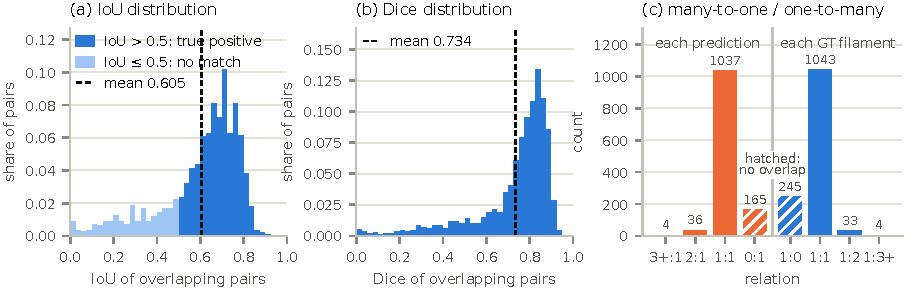
\includegraphics[width=\textwidth]{figures/fig_host_metrics.pdf}
\caption{The measures computed by the organisers' notebook on the final model's validation
predictions. (a) The IoU of every overlapping pair of annotation and prediction; the darker bars lie
above 0.5 and count as true positives. (b) The Dice coefficient of the same pairs. (c) How many
predictions touch each annotated filament (right), and how many filaments touch each prediction
(left); the hatched bars have no overlap at all. \generatedby{paper/make\_figures.py}}
\label{fig:sub-host}
\end{figure}

The results are summarised in the following table:
\begin{center}\small
\begin{tabular}{@{}lccc@{}}
\toprule
 & PQ & SQ & RQ \\
\midrule
final model, epoch 40 & \HostPQ{} & \ValSQ{} & \ValRQ{} \\
\quad 95\% bootstrap interval & [\PQLow{}, \PQHigh{}] & [\SQLow{}, \SQHigh{}] & [\RQLow{}, \RQHigh{}] \\
\quad TP / FP / FN & \multicolumn{3}{c}{\NumTP{} / \NumFP{} / \NumFN{}} \\
annotator against annotator & \HumanPQ{} & \HumanSQ{} & \HumanRQ{} \\
\quad 95\% bootstrap interval & [\HumanPQLow{}, \HumanPQHigh{}] & & \\
public leaderboard (test) & \BestPublic{} & -- & -- \\
\bottomrule
\end{tabular}
\end{center}
The intervals come from the bootstrap of Section~\ref{sec:metric-uncertainty}, which resamples the
\ValPhotos{} validation photographs 10,000 times, keeping the records of each photograph together. The
row for the annotators scores every annotator against every other annotator of the same validation
photographs, under the same rule. As Section~\ref{sec:metric-agreement} explained, the model's higher
score does not mean that it is more skilled than an expert. A model trained on many annotators learns
something like their average, and an average can lie closer to each person than two people lie to each
other.

Figure~\ref{fig:sub-host} adds the distributions that the organisers' notebook reports. The overlapping
pairs have a mean IoU of \MeanIoUOverlap{} and a mean Dice coefficient of \MeanDiceOverlap{}. Of the
annotated filaments, \GTOneOnePct{}\% touch exactly one prediction, \GTSplitPct{}\% touch two or more,
and \GTMissedPct{}\% touch none. Of the predictions, \PredOneOnePct{}\% touch exactly one filament,
\PredMergePct{}\% touch two or more, and \PredUnmatchedPct{}\% touch none.

In a reply in the competition's discussion forum, the host wrote that ``anything beyond 3.5 PQ is of
great interest to us''. Since PQ lies between 0 and 1, the number cannot be meant literally, and we have
recorded it as written without guessing what was intended. The same reply said that the judges will
look at individual predictions and at the logic of the algorithm, and not only at the score, and the
next section therefore looks at pictures.

\section{What the model gets right, and what it misses}\label{sec:sub-quality}
A summary number hides the individual predictions, so we now look at them. To avoid choosing a
flattering example, we selected the photograph for Figure~\ref{fig:sub-qual} by a fixed rule: among the
validation photographs that have a single annotator and at least eight filaments, it is the one whose
PQ is closest to the median. It is therefore a typical case.

\begin{figure}[t]
\centering
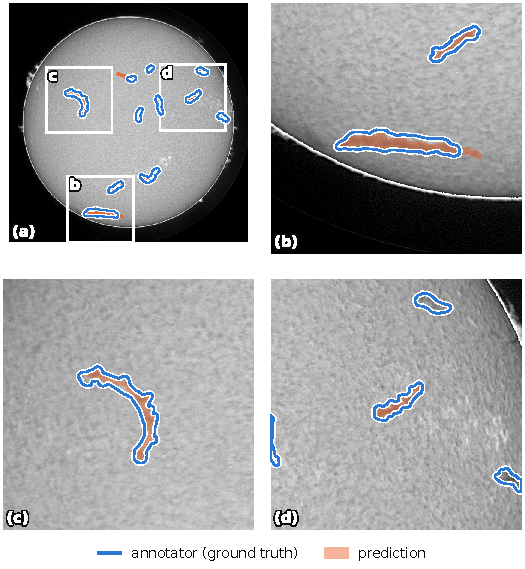
\includegraphics[width=\textwidth]{figures/fig_qualitative.pdf}
\caption{The validation photograph whose PQ (\QualPQ{}) is closest to the median of the
\QualCandidates{} single-annotator photographs with at least eight filaments (median \QualMedian{}).
(a) The full disk. (b)--(d) Zooms at the native resolution on the three largest annotated filaments.
Blue shows the annotation, outlined outside the mask so that the outline never covers it; orange shows
the model's prediction. \generatedby{paper/make\_figures.py}}
\label{fig:sub-qual}
\end{figure}

\paragraph{Strengths.} The model rarely splits or merges filaments: \GTSplitPct{}\% of the annotated
filaments touch more than one prediction, and \PredMergePct{}\% of the predictions touch more than one
filament. This is the set-prediction property of Section~\ref{sec:tr-detr} showing up in the counts.
Once a filament is found, its mask is good (SQ \ValSQ{}), and the boundaries follow the dark body without
the systematic widening that the early YOLO models needed erosion to remove. A review of validation
predictions at the native resolution, made before submission, found that the model detects large and
medium filaments reliably, including long curved ones. The whole test set runs in about
\TestMinutes{} minutes on one T4 GPU, at \SecondsPerPhoto{} seconds per photograph and with
\PeakGiB{} GiB of memory.

\paragraph{Weaknesses.} The model misses more than it invents, with \NumFN{} false negatives against
\NumFP{} false positives. Figure~\ref{fig:sub-size} shows where the misses occur. Recall is
\RecallSmall{} for the smallest sixth of the filaments (those under \SmallArea{} pixels) and
\RecallLarge{} for the largest sixth, and precision follows the same trend. The misses are concentrated
on thin, faint filaments, several of them next to bright active regions.

\begin{figure}[t]
\centering
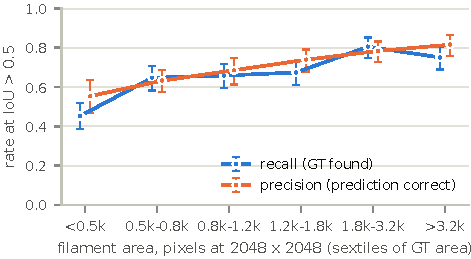
\includegraphics[width=0.7\textwidth]{figures/fig_size.pdf}
\caption{Recall (the fraction of annotated filaments found with an IoU above 0.5) and precision (the
fraction of predictions that match) as functions of filament area, in sixths of the annotated areas
(\PerBin{} filaments each). The bars are Wilson 95\% intervals (Section~\ref{sec:metric-uncertainty}).
\generatedby{paper/make\_figures.py}}
\label{fig:sub-size}
\end{figure}

Figure~\ref{fig:sub-failures} shows one example of each kind of error, again chosen by a fixed rule: the
median-sized filament that no prediction touches, the median-sized prediction that touches no filament,
and the largest filament that is touched by several predictions. The first is small and faint. The
second is a dark structure that this annotator did not mark, the kind of candidate that
Chapter~\ref{ch:recall} found so hard to judge. The third is a long filament covered in several pieces.

\begin{figure}[t]
\centering
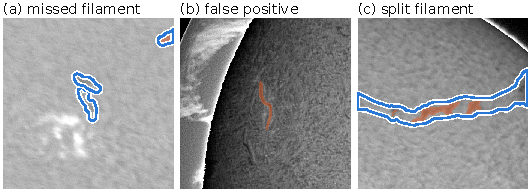
\includegraphics[width=\textwidth]{figures/fig_failures.pdf}
\caption{One example of each kind of error, chosen by a fixed rule over single-annotator validation
records: (a) the filament of median area that no prediction touches; (b) the prediction of median area
that touches no filament; (c) the largest filament touched by two or more predictions. The colours are as
in Figure~\ref{fig:sub-qual}. \generatedby{paper/make\_figures.py}}
\label{fig:sub-failures}
\end{figure}

\section{Variants that did not beat it}\label{sec:sub-variants}
We validated four variations of the final model and, to settle each question, submitted them:
\begin{center}\small
\begin{tabular}{@{}lcc@{}}
\toprule
variant & validation PQ & public \\
\midrule
\textbf{epoch 40, one view (deployed)} & \textbf{0.4705} & \textbf{0.41} \\
epoch 50, one view & 0.4621 & 0.40 \\
weight soup of epochs 40 and 50 & 0.4688 & 0.40 \\
epoch 40, eight-view fusion & 0.4700 & 0.40 \\
calibrated ensemble with YOLOv8l & 0.4715 & 0.40 \\
\bottomrule
\end{tabular}
\end{center}
Chapter~\ref{ch:tta} explained each of them. The last row is a useful warning. Its validation score
was 0.001 \emph{higher} than that of the deployed model, which is below the margin of 0.005 that we had
fixed in advance, and the leaderboard ranked it lower. Differences of this size cannot be resolved by
either instrument.

\section{What would come next}\label{sec:sub-next}
Our measurements point to three next steps. These are proposals, and we have no results for them yet.
\begin{enumerate}[leftmargin=*,itemsep=2pt]
\item \textbf{Train on every record.} The final model never saw the 180 validation records. With the
recipe fixed, a run on all 1,154 records would add 180 records to the 974 used so far, about 18\% more.
The division by zero that stopped the first attempt (Section~\ref{sec:train-run}) has been fixed, exact
gradient accumulation lets a card with 24 GB train the same model, and a measured speed of 1.34 seconds
per step on an RTX 3090 puts 30 epochs at a cost of about \$0.71. Without a held-out split, however,
such a run can be judged only by its training behaviour and by the leaderboard, so the recipe must be
frozen before the run starts.
\item \textbf{A gate for the extra detections.} Eight-view fusion added 60 true positives and 125 false
positives. By the arithmetic of Section~\ref{sec:recall-arith}, a verifier that kept two thirds of the
true positives and a third of the false positives would turn this into a gain. Chapter~\ref{ch:recall}
shows how hard such a verifier is to build, and why it must be labelled per record.
\item \textbf{Consensus targets.} There are 296 photographs with two or three annotations. An earlier
test found that a consensus of two annotators predicted a third no better than a single annotator did
(0.3291 against 0.3287), so consensus labels are not an obvious gain. Whether they help a model to
\emph{learn}, as opposed to scoring it, has never been tested.
\end{enumerate}

\section*{Exercises}
\begin{exercise}{Prefix painting}\label{ex:sub-prefix}
Prove that for any two thresholds $c_1 < c_2$, the painted set at $c_2$ equals the painted set at $c_1$
restricted to the candidates with scores of at least $c_2$, including the effect of the minimum-area
filter. Where would the proof break if painting gave contested pixels to the \emph{larger} mask
instead of the higher-scoring one?
\end{exercise}

\begin{exercise}{Reading the interval}
The bootstrap interval for the model's PQ is [\PQLow{}, \PQHigh{}], and the calibrated ensemble scored
0.4715. Explain why the two models cannot be ranked from these numbers, and what a paired bootstrap of
their difference would measure instead.
\end{exercise}

\begin{exercise}{Small filaments}
Using the recall and precision of the smallest sixth of the filaments, estimate how much PQ would rise
if the recall in that bin matched the recall in the largest bin, at the same precision and SQ. Compare
your estimate with the gains in Figure~\ref{fig:tta-ensembles}.
\end{exercise}

\begin{exercise}{Look before you submit}
Write a function that, for one photograph, draws the annotated outlines and the emitted masks on crops at
the native resolution around each of the three largest annotated filaments, as in
Figure~\ref{fig:sub-qual}. Why should the outlines be drawn outside the masks rather than on them?
\end{exercise}
